
\textbf{Asynchronous program execution as a stream of segments:} 

The execution of an asynchronous program can be decomposed into synchronous and asynchronous segments. An asynchronous segment is a code segment that runs asynchronously: an asynchronously called procedure  or a continuation segment (code segment below \emph{wait\_and\_return}). An asynchronously called procedure can run at any time and a continuation can run at any time after its antecedent task - of which it is the continuation of - is completed. A synchronous segment is a block of code that follows the conventional execution order. If a procedure does not involve any asynchronous segments, it returns to its caller after it completes its whole execution. If it contains some asynchronous segments (it has at least one \emph{wait\_and\_return} statements), the control returns to its caller at the first \emph{wait\_and\_return} point. The program execution continues from the synchronous segment of its caller. The asynchronous segment below \emph{wait\_and\_return} of the callee may resume at any point after the waited task is completed.\\
Basically, an asynchronous program runs two execution streams: one consisting of the synchronous segments and another consisting of the asynchronous ones. While there is a crucial ordering between the synchronous segments of an execution (due to the caller-callee relation), there is a notion of concurrency in the execution of asynchronous segments. The execution of asynchronous segments can interleave with the other ones in a way that the resulting execution is allowed by the semantics of the program (e.g. a continuation does not execute before its antecedent). 
Figure X.a shows the segments of an example asynchronous program and possible execution orders of these segments.
 
\vspace{4 mm}
\textbf{Sequencing order of segments in our method:}


Sequentialization of an asynchronous program sequences together the program segments in a way that it satisfies the constraints the various statements (e.g. call, async-call, wait, wait-and-return) put on the sequencing of those segments. We sequence the segments of a program such that all asynchronous segments come after the execution of the synchronous segments. The synchronous segments themselves are executed in their natural order due to the synchronous method calls. We simulate the execution order of asynchronous segments provided by our deterministic scheduler.  It yields an ordering of these segments so that they are collected and executed in their posting order. Such an ordering produces a sound execution since a continuation is posted (and hence, executed) after its antecedent task. \\
The execution of synchronous and asynchronous segments need to interleave when a synchronous procedure \emph{wait}s for a task. In that case, the execution of a waiting synchronous stream must continue after the execution of the asynchronous stream (the waited task was already posted into this stream). At waiting points, we consume the segments in the asynchronous stream and then, the execution of synchronous stream resumes.
Figure X shows the order of execution of the segments in example programs with/without \emph{wait}. 

\begin{figure}[H]
 \centering
 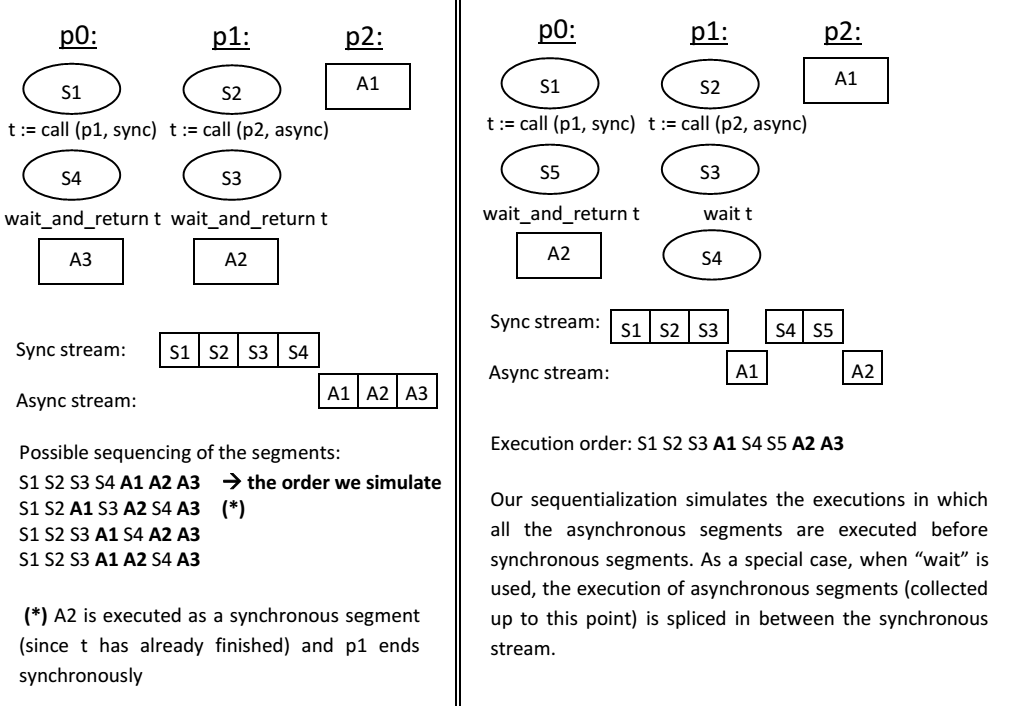
\includegraphics[scale=0.4]{segments.png}
 \caption{The synchronous and asynchronous segments in a program. On the left (a), the possible orders of execution of the segments allowed by the program semantics are given together with the ordering we simulate in our method. On the right (b), the order of execution we simulate is given on an example with \emph{wait} statement.}
 \label{figure:segments}
\end{figure}

\vspace{4 mm}
\textbf{Sequential encoding of an asynchronous program execution:} 

In our sequentialization, we simulate the execution of (i) a synchronous execution stream (consisting of synchronous segments) that starts with the initial global state \emph{g0}, updates the current state\emph{g} during its execution and (ii) virtual asynchronous execution stream (consisting of asynchronous segments) that starts with a guessed \emph{async.head} state and ends with \emph{async.tail}. This stream is called \textit{virtual} since it executes on a guessed global state.

\emph{async.head} is guessed nondeterministically in the beginning of the program, which is initially equal to \emph{async.tail}. An asynchronous segment starts execution in \emph{async.tail} state and updates to the state that it completes its execution. 
The guessed \emph{async.head} is verified at the end of the synchronous stream execution (asynchronous stream begins its execution after the execution of the synchronous stream). This state can be either the state at (i) the last \emph{wait\_and\_return} statement of the program (the end of whole synchronous stream) or (ii) a wait statement (pause the execution of synchronous stream and execute the asynchronous stream).

At \emph{wait} points, after verifying the \emph{async.head}, current state is set to \emph{async.tail} to resume the execution of synchronous stream after the execution of all segments in asynchronous stream. A new \emph{async.head} is guessed which is the initial state of a next asynchronous segment and will be verified at a pause/end of the synchronous segment.
 
At a \emph{wait\_and\_return}, the segment involving the rest of the code (the continuation segment) is enqueued into the asynchronous stream (if the waited task is not completed). As for the other asynchronous segments, its execution starts with \emph{async.tail}, it guesses a new \emph{async.tail} state and verifies it end the end of its execution. 

In addition to the global variables \emph{g}, \emph{async.head} and \emph{async.tail}, we use two additional local variables \emph{guess} and \emph{save} in the encoding: 

\begin{itemize}
\item {var g : G - stores the current global state}
\item {var async.head : G - stores the global state where a sequence of asynchronous segments began}
\item {var async.tail : G - stores the global state reached by a sequence of asynchronous segments}

\item {var \emph{guess} : G - keeps the guessed \emph{async.tail} state and used to verify the guess with the state after execution.}
\item{var \emph{save} : G - keeps the state to be returned to the caller of a procedure. An asynchronously called procedure saves the current state before its execution and restores it back before it returns, to simulate the uninterrupted execution of the calling procedure.  An asynchronously returning procedure saves the state at which it will return the control to the caller (i.e. before the first \emph{wait\_and\_return} of a synchronously called procedure) and restores it back before it returns.}
\end{itemize}

The encoding extends a procedure declaration with an additional boolean \emph{isSync} parameter. It is called with $isSync := true$, when a procedure is called synchronously, with $isSync := false$ when it is called asynchronously. An asynchronously called (posted) procedure ends asynchronously, where a synchronously called procedure can end either synchronously (as a conventional procedure call) or asynchronously. A synchronously called method ends asynchronously if it \emph{wait\_and\_returns} for an incomplete task. In that case, \emph{isSync} is set to false and it returns the control to its caller before it completes its execution. 

\begin{figure}
\vspace{-2ex}
\begin{scriptsize}
\begin{multicols}{2}
\begin{verbatim}
// translation of declaration var g: G
var g, async.head, async.tail : G

// translation of 'proc p(x:T) s'
proc p(x:T, isSync: bool)
    var save: G
    var guess: G
    
    if !isSync then
        // end the synchronous segment
        save := g;
        
        // begin an asynchronous segment
        g := async.tail;
        async.tail := guess := *;
    end;
    s
end

// translation of 'call x := p e'
call x := p(e,true)

// translation of 'async t := p e'
call t := p(e,true)

// translation of 'post t := p e'
call t := p(e,false)

// translation of 'return e'
let v := e in
if !isSync then
    // end asynchronous segment
    // (validate guessed async.tail)
    assume g = guess;
    
    // resume synchronous segment
    g := save;
end;
return { val: v, ready: isSync }

// translation of 'wait_and_return x := t'
if !t.ready then

    if isSync then
        // end the synchronous segment
        save := g;
        isSync := false;
    else
        // end an asynchronous segment
        assume g = guess;
    end;
    
    // begin an asynchronous segment
    g := async.tail;
    async.tail := guess := *;
    
    // all *visited* tasks have completed
    for each t' in scope
        t'.ready := true
    end;
end;
x := t.val

// translation of 'wait x := t'
if !t.ready then

    // consume asynchronous stream
    assume g = async.head;

    // resume synchronous execution 
    // where async stream has finished
    g := async.tail;

    // guess a new async start state 
    async.head := async.tail := guess := *; 
    
    // all *visited* tasks have completed
    for each t' in scope
        t'.ready := true
    end;
end;

// translation of 'yield'
skip  

// top entry procedure to execute P
proc Main(var l : G)
    g := g0;
    t := call P(l, true);
    
    // async stream starts where
    // the sync stream is completed
    assume g = async.head;
    return;
end

\end{verbatim}
\end{multicols}
\end{scriptsize}
\vspace{-1ex}
\caption{No-delay translation of a program P}
\label{fig:seq_no_delay}
\vspace{-2ex}
\end{figure}




